\clearpage
\section{Video}
\subsection{Throughput}
For a video feed of resolution $W*H$, $B$ bits per pixel and $F$ frames per second the required bandwidth is given by the product of the terms
\[
    H * W * B * F
\]

This number may grow very quickly when increasing some of the terms.
It was clear from the beginning that we would no be able to output full HD video,
but it was not not clear what exactly the limits would be, nor where the bottlenecks would be located.

The Raspberry Pi camera can output resolutions and framerates based on commands from the master device.
It may output encoded video, but this would have to be decoded before convolution,
so it was decided to go with 24-bit raw RGB as camera output.

\subsection{Options for Video Path}
There were several options for how to move the video stream to the processor.

\begin{figure}[h]
    \centering
    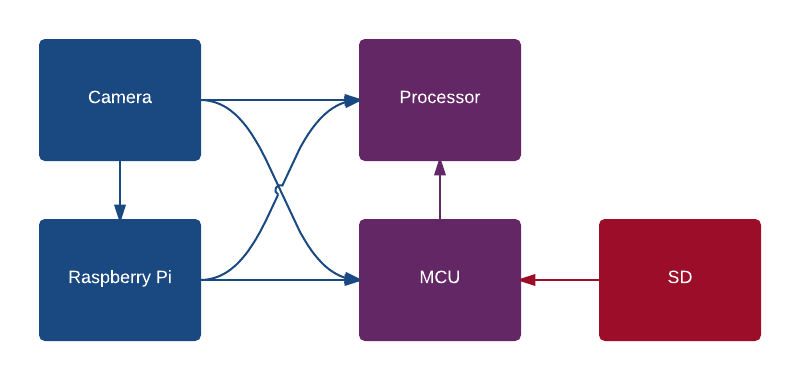
\includegraphics[width=\linewidth]{img/VideoPath}
    \caption{Paths an input video stream could take to reach the processor.}
    \label{fig:VideoPath}
\end{figure}

\subsubsection{Direct Path from Camera to Processor}
The path with the fewest bottleneck would be to send data directly from the camera to the processor.
This would also mean that the FPGA would have to act as the camera master,
sending control signals over I2C.

\subsubsection{Camera to MCU to Processor}
The signals from the camera could also be routed to the MCU.
This would mean that the MCU would be the camera master,
leaving the FPGA free to work on other problems.
Another advantage of this is that the processor would not need to mode-switch between SD and camera input,
since the MCU would handle this.

\subsubsection{Using the Raspberry Pi as Camera Controller}
Instead of reverse-engineering the camera control protocol,
the system could include a whole Raspberry Pi with a camera as the camera module.
Programming the Pi to start recording is very easy thanks to the provided software.
However the video stream would then have to be outputted from the Pi to the Camvolution computer somehow,
which would introduce a considerable bottleneck.

\subsubsection{GPIO}
Software was written for the Pi which started recording then used the Pi GPIO pins as a clocked parallell bus to output color values.
Getting this program to work was not very difficult,
however it was very slow.

\subsubsection{HDMI}
The Pi has an HDMI output.
Since the Camvolution board has two HDMI ports,
it would be possible to output video from the Pi to Camvolution over HDMI.
This would require a HDMI decoding module to be implemented on Camvolution.

